% Figure of the starter beamer deck (scripts/gen-starters.ts compiles it to templates/starters/slides/figures/decay.pdf).
\documentclass[border=2pt]{standalone}
\usepackage[T1]{fontenc}
\usepackage[scaled]{helvet}
\renewcommand{\familydefault}{\sfdefault}
\usepackage{sansmath}
\usepackage{pgfplots}
\pgfplotsset{compat=1.18}
\begin{document}
\sansmath
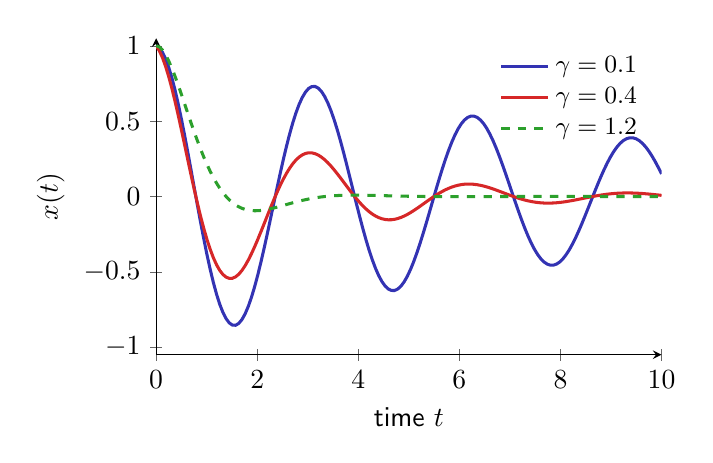
\begin{tikzpicture}
\begin{axis}[width=8cm, height=5.6cm, xmin=0, xmax=10, ymin=-1.05, ymax=1.05,
  xlabel={time $t$}, ylabel={$x(t)$}, axis lines=left, tick style={black!60},
  legend style={draw=none, font=\small, fill=none, at={(0.98,0.98)}, anchor=north east},
  every axis plot/.append style={line width=1.1pt, samples=160, domain=0:10}]
\addplot[color={rgb,255:red,51;green,51;blue,179}] {exp(-0.1*x)*cos(deg(2*x))};
\addplot[color={rgb,255:red,214;green,39;blue,40}] {exp(-0.4*x)*cos(deg(2*x))};
\addplot[color={rgb,255:red,44;green,160;blue,44}, dashed] {exp(-1.2*x)*(cos(deg(1.6*x))+0.75*sin(deg(1.6*x)))};
\legend{$\gamma=0.1$, $\gamma=0.4$, $\gamma=1.2$}
\end{axis}
\end{tikzpicture}
\end{document}
